\chapter{Théorie des réseaux de neurones}     
\label{chap:RN}                   

\section{Apprentissage supervisé}
\label{sec:RN:ML}

La section présente est basée sur le chapitre 2 de \citet{james2013introduction} et le chapitre 2 de \citet{Hastie/etal:2009}.

Les réseaux de neurones sont des modèles qui peuvent s'appliquer tant à l'apprentissage supervisé qu'à l'apprentissage non-supervisé. On résume dans cette section les bases de l'apprentissage supervisé pour la suite.

Soit $X=\left(X_1, \dots X_p \right)$, un vecteur de $p$ variables aléatoires et $Y$, une variable que l'on veut prédire. On suppose qu'il existe une relation entre $Y$ et $X$ telle que,

\begin{align*}
Y = f(X) + \epsilon,
\end{align*} 

où $f$ est une fonction quelconque et $\epsilon$ est un terme d'erreur qui est indépendant de $X$. L'apprentissage supervisé vise à estimer $f$ pour pouvoir prédire et/ou expliquer $Y$ à partir de $X$. On veut utiliser les données pour estimer une fonction $f$ qui soit utile, c'est-à-dire, une fonction qui permet de bien estimer $Y$ à partir de nouvelles données. 

Un algorithme d'apprentissage supervisé est capable de modifier ses paramètres internes en réponse à une fonction objective. En d'autres termes, il apprend à partir des erreurs commises.  La fonction objective mesure donc la différence entre la prédiction, $\hat{f}(x)$, et la vraie valeur de $Y$. On dénote cette fonction par 

\begin{align*}
\mathcal{L} \left( Y, \hat{f}(X) \right)= \left( \hat{f}(X) - Y\right)^2.
\end{align*}

\subsection{Compromis biais-variance}
\label{subsec:RN:ML:biais-var}

Un des enjeux principaux en apprentissage statistique est le compromis biais-variance. On veut un modèle qui soit le plus précis possible tout en étant le moins variable possible. Par contre, lorsqu'on diminue le biais, la variance de l'estimateur finit toujours par augmenter: on doit trouver le compromis. On illustre cet enjeu par l'erreur quadratique espérée:

\begin{align*}\mathrm{E}\left[\left\{Y_{0}-\hat{f}\left(X\right)\right\}^{2}\right]=\operatorname{Biais}^{2}\left\{\hat{f}\left(X\right)\right\}+\operatorname{var}\left\{\hat{f}\left(X\right)\right\}+ \sigma^{2},
\end{align*}
où $\sigma^2=\operatorname{var}\left(\epsilon\right)$, l'erreur irréductible.

On ne peut pas diminuer l'erreur irréductible, comme son nom l'indique, puisqu'elle fait partie de tout processus aléatoire. Toutefois, on peut diminuer l'erreur réductible (biais + variance) en diminuant ou en augmentant la complexité du modèle. La complexité du modèle se traduit par le nombre de paramètres qu'il faut estimer. Plus on a de paramètres, plus le modèle est en mesure de faire des prédictions exactes sur les données d'entrainement. En revanche, la variance sera plus élevée, car le modèle aura appris les caractéristiques  des observations qui sont propres à celles-ci. 

Pour être en mesure de surveiller le compromis, on sépare les données en trois échantillons distincts: l'échantillon d'entrainement, l'échantillon de validation et l'échantillon de test. L'échantillon d'entrainement $\mathcal{D}$ est celui sur lequel on entraine le modèle; il sert à ajuster les paramètres. L'échantillon de test $\mathcal{T}$ permet de mesurer la performance du modèle et ainsi le comparer avec d'autres. L'échantillon de validation $\mathcal{V}$ permet de faire la sélection d'hyperparamètres et c'est à partir de celui-ci qu'on surveille si le modèle ne surajuste pas les données d'entrainement. 

\begin{figure}[h]
\centering
\caption{\label{fig:ErrPredVsComplex}Erreur de prédiction en fonction de la complexité du modèle}
\includegraphics[height=8cm,width=10cm]{Rplot_prederror_complexité}
\end{figure}

La \autoref{fig:ErrPredVsComplex} montre un example de l'erreur de prédiction en fonction de la complexité d'un modèle. On voit que plus la complexité augmente, plus l'erreur de prédiction sur les données d'entrainement diminue. On remarque, aussi, que l'erreur de prédiction sur les données de validation diminue lorsqu'on augmente la complexité pour ensuite augmenter. Lorsque le modèle atteint le point où l'erreur de prédiction sur l'échantillon de validation augmente, on dit que le modèle surajuste l'échantillon d'entrainement. Il ne généralise pas bien pour des données qu'il n'a pas vu. L'objectif devient donc de trouver une combinaison des paramètres à estimer et de la complexité du modèle pour minimiser la fonction objective sur l'échantillon de validation.

\section{Architecture d'un réseau de neurones}
\label{sec:RN:architecture}

Malgré qu'il existe plusieurs types de réseau de neurones, la section présente ainsi que l'analyse de données subséquente sont basées sur la forme la plus simple de réseau de neurones, soit le perceptron ou réseau de neurones à propagation directe (« feedforward neural network »). Il existe deux formes de perceptron: le perceptron simple et le perceptron multicouche.  La différence entre les deux formes réside dans le nombre de couche cachée. Le perceptron simple a une seule couches cachées, tandis que le perceptron multicouche en a plusieurs. Pour bien comprendre le perceptron, on compare son fonctionnement avec des modèles plus simples. On illustre les modèles de régression linéaire simple et multiple et le modèle de régression logistique pour expliquer la progression qui nous amènera au réseau de neurones.

\def\layersep{2.5cm}

\begin{figure}[h]
\centering
\caption{\label{fig:reglin}Modèle de régression linéaire simple}
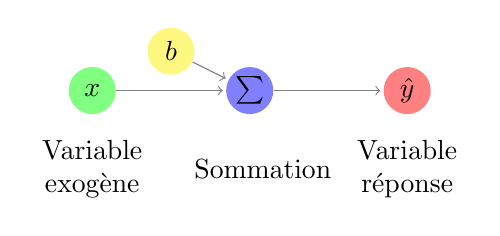
\begin{tikzpicture}[shorten >=1pt,->,draw=black!50, node distance=\layersep]
    \tikzstyle{every pin edge}=[<-,shorten <=1pt]
    \tikzstyle{neuron}=[circle,fill=black!25,minimum size=17pt,inner sep=0pt]
    \tikzstyle{input neuron}=[neuron, fill=green!50];
    \tikzstyle{output neuron}=[neuron, fill=red!50];
    \tikzstyle{hidden neuron}=[neuron, fill=blue!50];
    \tikzstyle{bias}=[neuron, fill=yellow!50];
    \tikzstyle{annot} = [text width=4em, text centered]

    % Draw the input layer nodes
        \node[input neuron] (I-1) at (0,-1) {$x$};
        
	%Bias node
	\node[bias] (B1) at (0.5*\layersep,-0.5 cm) {$b$};	        

    % Draw the hidden layer nodes
   	\node[hidden neuron] (S-1) at (\layersep,-1 cm) {$\sum$};

	
	% Draw the output layer node, first the sum then the response
	\node[output neuron] (O) at (2*\layersep,-1 cm) {$\hat{y}$};

    
   

    % Connect every node in the input layer with every node in the
    % sum layer.
            \path (I-1) edge (S-1);
	
	% Connect les biais avec les sommes
            \path (B1) edge (S-1);
            
	% Connect every node in the sum layer with every node in the
    % hidden layer.
            
    % Connect every node in the hidden layer with the output sum layer

        \path (S-1) edge (O);
	
	
    % Annotate the layers
    \node[annot,below of=I-1, node distance=1cm] (i1) {Variable exogène};
    \node[annot,right of=i1, node distance=\layersep] (hid1) {Sommation};
    \node[annot,right of=hid1,node distance=\layersep] {Variable réponse};
\end{tikzpicture}
\end{figure}

Un modèle de régression linéaire simple est une somme de la variable exogène. On suppose que la relation entre $Y$ et $X$ est de la forme suivante:
\begin{align*}
Y = b+\omega X + \epsilon.
\end{align*}
On estime $Y$ par
\begin{align*}
\hat{Y} = \hat{f} (X) = \hat{b}+\hat{\omega} X.
\end{align*}
Ce modèle utilise l'information qui est contenue dans la variable exogène pour prédire la variable réponse. Pour ce faire, on calcule $\hat{b}$ et $\hat{\omega}$ de façon à minimiser l'erreur quadratique de prévision.  
On illustre ce modèle à l'aide 
de la \autoref{fig:reglin}. La partie verte de la figure illustre l'information qui entre dans le modèle, la partie bleue est le traitement de l'information et la partie rouge est la prévision du modèle. On voit que la partie bleue est en fait la fonction $\hat{f}$. Le terme de la partie jaune est le biais. 

\begin{figure}[h]
\centering
\caption{\label{fig:reg:lin:mult}Modèle de régression multiple}
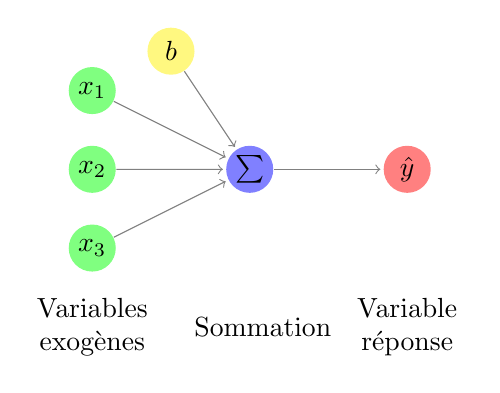
\begin{tikzpicture}[shorten >=1pt,->,draw=black!50, node distance=\layersep]
    \tikzstyle{every pin edge}=[<-,shorten <=1pt]
    \tikzstyle{neuron}=[circle,fill=black!25,minimum size=17pt,inner sep=0pt]
    \tikzstyle{input neuron}=[neuron, fill=green!50];
    \tikzstyle{output neuron}=[neuron, fill=red!50];
    \tikzstyle{hidden neuron}=[neuron, fill=blue!50];
    \tikzstyle{bias}=[neuron, fill=yellow!50];
    \tikzstyle{annot} = [text width=4em, text centered]

    % Draw the input layer nodes
    \foreach \name / \y in {1,...,3}
    % This is the same as writing \foreach \name / \y in {1/1,2/2,3/3,4/4}
        \node[input neuron] (I-\name) at (0,-\y) {$x_{\y}$};
        
	%Bias node
	\node[bias] (B1) at (0.5*\layersep,-0.5 cm) {$b$};	        

    % Draw the hidden layer nodes
    \node[hidden neuron] (S-1) at (\layersep,-2 cm) {$\sum$};
	
	% Draw the output layer node, first the sum then the response    	
    	\node[output neuron] (O) at (2*\layersep,-2 cm) {$\hat{y}$};

    
   

    % Connect every node in the input layer with every node in the
    % sum layer.
    \foreach \source in {1,...,3}
            \path (I-\source) edge (S-1);
	
	% Connect les biais avec les sommes
    \path (B1) edge (S-1);
            
	% Connect every node in the sum layer with every node in the
    % hidden layer.
    \path (S-1) edge (O);

	
	
    % Annotate the layers
    \node[annot,below of=I-3, node distance=1cm] (i1) {Variables exogènes};
    \node[annot,right of=i1, node distance=\layersep] (hid1) {Sommation};
    \node[annot,right of=hid1,node distance=\layersep] {Variable réponse};
\end{tikzpicture}
\end{figure} 

Dans le cas de la régression linéaire multiple, on a plusieurs variables exogènes. On fait une sommation pondérée de toutes ces variables pour pouvoir prédire la variable réponse. La relation entre Y et X est
\begin{align*}
Y = b + \sum_{i=1}^n \omega_{i} X_i + \epsilon.
\end{align*}

On estime Y par

\begin{align*}
\hat{Y} = \hat{f} (X) = \hat{b}+\sum_{i=1}^n \hat{\omega}_{i} X_i.
\end{align*}

 La \autoref{fig:reg:lin:mult} illustre un cas avec 3 variables exogènes. On y voit le même mécanisme 
qu'avec la régression linéaire simple, c'est-à-dire, on combine l'information, on la traite et puis on prédit un résultat. La différence est que l'information a plus d'une dimension. On doit donc estimer un paramètre pour chaque variable exogène et un paramètre pour le biais. Il s'en dégage une structure qui est bien présente dans les modèles d'apprentissage statistique. 


\begin{figure}[h]
\centering
\caption{\label{fig:reg:log}Régression logistique}
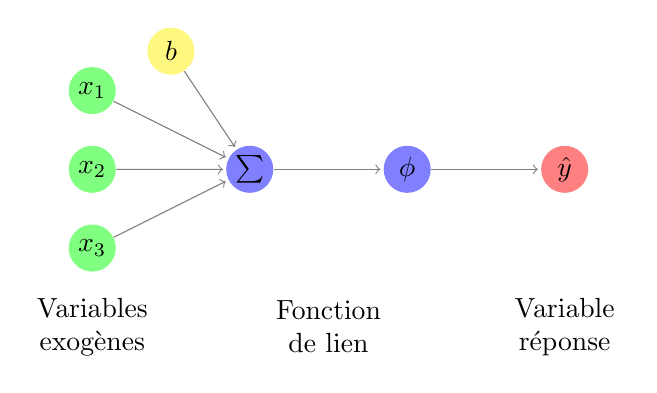
\begin{tikzpicture}[shorten >=1pt,->,draw=black!50, node distance=\layersep]
    \tikzstyle{every pin edge}=[<-,shorten <=1pt]
    \tikzstyle{neuron}=[circle,fill=black!25,minimum size=17pt,inner sep=0pt]
    \tikzstyle{input neuron}=[neuron, fill=green!50];
    \tikzstyle{output neuron}=[neuron, fill=red!50];
    \tikzstyle{hidden neuron}=[neuron, fill=blue!50];
    \tikzstyle{bias}=[neuron, fill=yellow!50];
    \tikzstyle{annot} = [text width=4em, text centered]

    % Draw the input layer nodes
    \foreach \name / \y in {1,...,3}
    % This is the same as writing \foreach \name / \y in {1/1,2/2,3/3,4/4}
        \node[input neuron] (I-\name) at (0,-\y) {$x_{\y}$};
        
	%Bias node
	\node[bias] (B1) at (0.5*\layersep,-0.5 cm) {$b$};	        

    % Draw the hidden layer nodes

    \node[hidden neuron] (S-1) at (\layersep,-2 cm) {$\sum$};
            
    \node[hidden neuron] (H-1) at (2*\layersep,-2 cm) {$\phi$};

	
	% Draw the output layer node, first the sum then the response
    	
    	\node[output neuron] (O) at (3*\layersep,-2 cm) {$\hat{y}$};

    
   

    % Connect every node in the input layer with every node in the
    % sum layer.
    \foreach \source in {1,...,3}
            \path (I-\source) edge (S-1);
	
	% Connect les biais avec les sommes
            \path (B1) edge (S-1);
            
	% Connect every node in the sum layer with every node in the
    % hidden layer.
            \path (S-1) edge (H-1);
            
    % Connect every node in the hidden layer with the output sum layer
        \path (H-1) edge (O);
	
	
    % Annotate the layers
    \node[annot,below of=I-3, node distance=1cm] (i1) {Variables exogènes};
    \node[annot,right of=i1, node distance=\layersep + 0.5*\layersep] (hid1) {Fonction de lien};
    \node[annot,right of=hid1,node distance=1.5*\layersep] {Variable réponse};
\end{tikzpicture}
\end{figure}

La régression logistique, quant à elle, ajoute une transformation non-linéaire à la combinaison linéaire des variables exogènes. Ainsi, la variable prédite peut être contenue dans l'espace $[0,1]$. La \autoref{fig:reg:log} ajoute donc $\phi$ au traitement de l'information. Le modèle est

\begin{align*}
Y = \frac{e^{b+ \sum_{i=1}^n \omega_{i} X_i}}{1+e^{b+ \sum_{i=1}^n \omega_{i} X_i}}.
\end{align*}

La relation entre Y et X est ainsi non-linéaire. On peut voir la régression logistique comme étant un réseau de neurones avec une seule couche cachée et un seul neurone dans la couche cachée. 

\begin{figure}[h]
	\centering
	\caption[Réseau de neurones avec une couche cachée]{\label{fig:NNsimple}Réseau de neurones avec une couche cachée\footnotemark} 
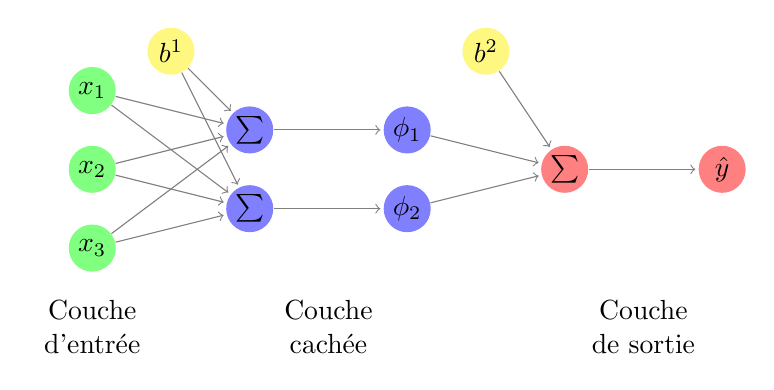
\begin{tikzpicture}[shorten >=1pt,->,draw=black!50, node distance=\layersep]
    \tikzstyle{every pin edge}=[<-,shorten <=1pt]
    \tikzstyle{neuron}=[circle,fill=black!25,minimum size=17pt,inner sep=0pt]
    \tikzstyle{input neuron}=[neuron, fill=green!50];
    \tikzstyle{output neuron}=[neuron, fill=red!50];
    \tikzstyle{hidden neuron}=[neuron, fill=blue!50];
    \tikzstyle{bias}=[neuron, fill=yellow!50];
    \tikzstyle{annot} = [text width=4em, text centered]

    % Draw the input layer nodes
    \foreach \name / \y in {1,...,3}
    % This is the same as writing \foreach \name / \y in {1/1,2/2,3/3,4/4}
        \node[input neuron] (I-\name) at (0,-\y) {$x_{\y}$};
        
	%Bias node
	\node[bias] (B1) at (0.5*\layersep,-0.5 cm) {$b^{1}$};	        

    % Draw the hidden layer nodes
    \foreach \name / \y in {1,...,2}
        \path[yshift=-0.5cm]
            node[hidden neuron] (S-\name) at (\layersep,-\y cm) {$\sum$};
            
    \foreach \name / \y in {1,...,2}
        \path[yshift=-0.5cm]
            node[hidden neuron] (H-\name) at (2*\layersep,-\y cm) {$\phi_{\y}$};

	% Draw les biais pour la somme output
	\node[bias] (B2) at (2.5*\layersep,-0.5 cm) {$b^{2}$};	
	
	% Draw the output layer node, first the sum then the response
    	\node[output neuron] (OS) at (3*\layersep,-2 cm) {$\sum$};
    	
    	\node[output neuron] (O) at (4*\layersep,-2 cm) {$\hat{y}$};

    
   

    % Connect every node in the input layer with every node in the
    % sum layer.
    \foreach \source in {1,...,3}
        \foreach \dest in {1,...,2}
            \path (I-\source) edge (S-\dest);
	
	% Connect les biais avec les sommes
	\foreach \dest in {1,...,2}
            \path (B1) edge (S-\dest);
            
	% Connect every node in the sum layer with every node in the
    % hidden layer.
	\foreach \source in {1,...,2}
            \path (S-\source) edge (H-\source);
            
    % Connect every node in the hidden layer with the output sum layer
    \foreach \source in {1,...,2}
        \path (H-\source) edge (OS);
	
	% Connect bias with the output sum layer
	\path (B2) edge (OS);
	
	% Connect every node in the hidden layer with the output sum layer
	\path (OS) edge (O);
	
    % Annotate the layers
    \node[annot,below of=I-3, node distance=1cm] (i1) {Couche d'entrée};
    \node[annot,right of=i1, node distance=\layersep + 0.5*\layersep] (hid1) {Couche cachée};
    \node[annot,right of=hid1,node distance=2*\layersep] {Couche de sortie};
\end{tikzpicture}
\end{figure}

\footnotetext{Ce graphique est une adaptation de la réponse de l'utilisateur \emph{gvgramazio} sur \url{https://tex.stackexchange.com/questions/153957/drawing-neural-network-with-tikz}}

Les trois exemples précédents permettent de voir que les réseaux de neurones ne sont en fait qu'une généralisation de la régression linéaire. En effet, comme le montre la \autoref{fig:NNsimple}, la partie de traitement de l'information(en bleu) est constituée de plusieurs neurones(deux neurones dans cet exemple). À chaque neurone, on combine linéairement les variables exogènes et on applique la fonction d'activation $\phi$. Ensuite, la combinaison linéaire de la réponse de chacun de ces neurones est utilisée pour prédire la variable réponse du réseau. Chaque résultat des fonctions $\phi$ deviennent à leur tour de nouvelles variables entrant dans un réseau. Illustrons ceci par un exemple.

\begin{figure}[h]
	\centering
	\caption{\label{fig:TransfoNNsimple}Décomposition d'un réseau en une suite de deux réseaux} 
\def\layersep{2cm}
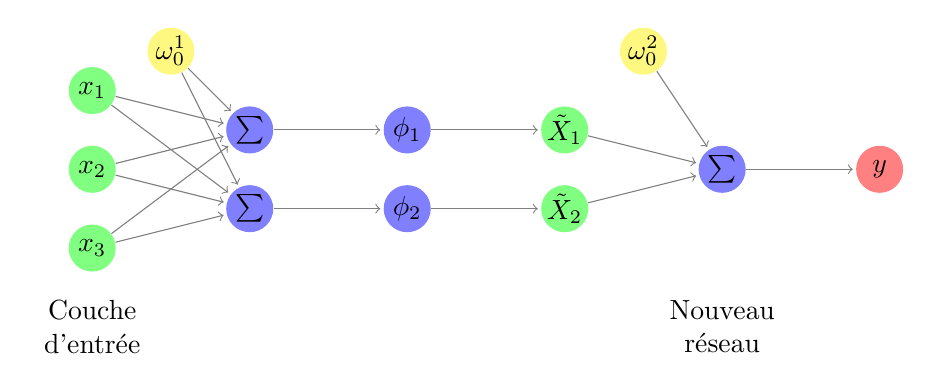
\begin{tikzpicture}[shorten >=1pt,->,draw=black!50, node distance=\layersep]
    \tikzstyle{every pin edge}=[<-,shorten <=1pt]
    \tikzstyle{neuron}=[circle,fill=black!25,minimum size=17pt,inner sep=0pt]
    \tikzstyle{input neuron}=[neuron, fill=green!50];
    \tikzstyle{output neuron}=[neuron, fill=red!50];
    \tikzstyle{hidden neuron}=[neuron, fill=blue!50];
    \tikzstyle{bias}=[neuron, fill=yellow!50];
    \tikzstyle{annot} = [text width=4em, text centered]

    % Draw the input layer nodes
    \foreach \name / \y in {1,...,3}
    % This is the same as writing \foreach \name / \y in {1/1,2/2,3/3,4/4}
        \node[input neuron] (I-\name) at (0,-\y) {$x_{\y}$};
        
	%Bias node
	\node[bias] (B1) at (0.5*\layersep,-0.5 cm) {$\omega_0^{1}$};	        

    % Draw the hidden layer nodes
    \foreach \name / \y in {1,...,2}
        \path[yshift=-0.5cm]
            node[hidden neuron] (S-\name) at (\layersep,-\y cm) {$\sum$};
            
    \foreach \name / \y in {1,...,2}
        \path[yshift=-0.5cm]
            node[hidden neuron] (H-\name) at (2*\layersep,-\y cm) {$\phi_{\y}$};
            
	\foreach \name / \y in {1,...,2}
        \path[yshift=-0.5cm]
            node[input neuron] (HI-\name) at (3*\layersep,-\y cm) {$\tilde{X}_{\y}$};


	% Draw les biais pour la somme output
	\node[bias] (B2) at (3.5*\layersep,-0.5 cm) {$\omega_0^{2}$};	
	
	% Draw the output layer node, first the sum then the response
    	\node[hidden neuron] (OS) at (4*\layersep,-2 cm) {$\sum$};
    	
    	\node[output neuron] (O) at (5*\layersep,-2 cm) {$y$};

    
   

    % Connect every node in the input layer with every node in the
    % sum layer.
    \foreach \source in {1,...,3}
        \foreach \dest in {1,...,2}
            \path (I-\source) edge (S-\dest);
	
	% Connect les biais avec les sommes
	\foreach \dest in {1,...,2}
            \path (B1) edge (S-\dest);
            
	% Connect every node in the sum layer with every node in the
    % hidden layer.
	\foreach \source in {1,...,2}
            \path (S-\source) edge (H-\source);
            
    % Connect every node in the hidden layer with the output sum layer
    \foreach \source in {1,...,2}
        \path (H-\source) edge (HI-\source);
	
	\foreach \source in {1,...,2}
        \path (HI-\source) edge (OS);
	% Connect bias with the output sum layer
	\path (B2) edge (OS);
	
	% Connect every node in the hidden layer with the output sum layer
	\path (OS) edge (O);
	
    % Annotate the layers
    \node[annot,below of=I-3, node distance=1cm] (i1) {Couche d'entrée};
    \node[annot,right of=i1,node distance= 4*\layersep] (hid1) {Nouveau réseau};
    %\node[annot,right of=hid1,node distance=2*\layersep] {Couche de sortie};
\end{tikzpicture}
\end{figure}

La \autoref{fig:TransfoNNsimple} montre que les fonctions non-linéaires $\phi_j$ créent une nouvelle représentation de l'information. Cette représentation est alors combinée linéairement et traitée par un autre réseau. On voit que l'on peut reproduire cette séquence un nombre indéfini de fois. Par mesure de simplicité et pour ne pas saturer les graphiques, on résume chaque neurone par $a_j^1 = \phi_j \left(b^1 + \sum_{i=1}^n \omega_i^1 X_i \right)$, pour le $j$ième neurone de la première couche cachée, et par $a_j^l  = \phi \left( b_j^l+ \sum_{k=1}^{q_{k-1}} \omega_{j,k}^l a_k^{l-1} \right)$, pour le $j$ième neurone de la $l$ième couche cachée. On a $q_k$ neurones pour la $k$ième couche cachée. La \autoref{fig:NN:Deep2} illustre un réseau de neurones en considérant cette notation avec deux couches cachées de quatre et trois neurones, respectivement. On remarque une neurone supplémentaire directement lié à la prévision, soit $a_1^3$ dans notre exemple, ou $z_1^{l+1}$ pour un réseau avec $k$ couches cachées et une seule prédiction. Ce dernier neurone permet de faire le lien entre entre le réseau et la prévision. C'est la fonction de régression. 

\begin{figure}[h]
	\centering
	\caption{\label{fig:NN:Deep2}Réseau de neurones avec deux couches cachées} 
\def\layersep{2cm}
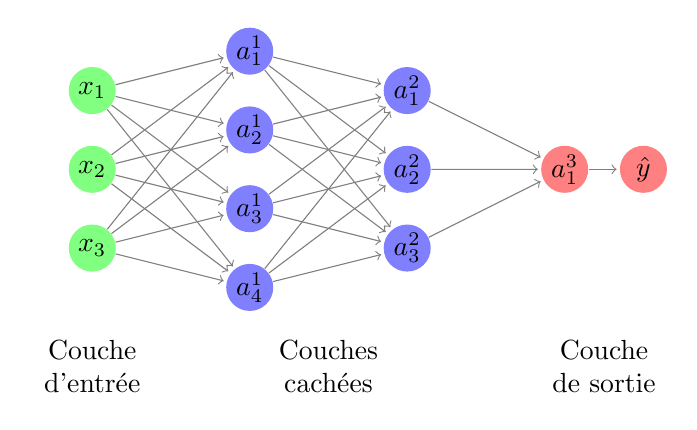
\begin{tikzpicture}[shorten >=1pt,->,draw=black!50, node distance=\layersep]
    \tikzstyle{every pin edge}=[<-,shorten <=1pt]
    \tikzstyle{neuron}=[circle,fill=black!25,minimum size=17pt,inner sep=0pt]
    \tikzstyle{input neuron}=[neuron, fill=green!50];
    \tikzstyle{output neuron}=[neuron, fill=red!50];
    \tikzstyle{hidden neuron}=[neuron, fill=blue!50];
    \tikzstyle{bias}=[neuron, fill=yellow!50];
    \tikzstyle{annot} = [text width=4em, text centered]

    % Draw the input layer nodes
    \foreach \name / \y in {1,...,3}
    % This is the same as writing \foreach \name / \y in {1/1,2/2,3/3,4/4}
        \path[yshift=-0.5cm] node[input neuron] (I-\name) at (0,-\y) {$x_{\y}$};
    %Première couche 4 neurones             
    \foreach \name / \y in {1,...,4}
            \node[hidden neuron] (H-\name) at (\layersep,-\y cm) {$a_{\y}^1$};
    %Deuxième couche 3 neurones
	\foreach \name / \y in {1,...,3}
        \path[yshift=-0.5cm]
            node[hidden neuron] (H2-\name) at (2*\layersep,-\y cm) {$a_{\y}^2$};
    	
    	\node[output neuron] (OA) at (3*\layersep, -2.5 cm) {$a_{1}^3$};
    	\node[output neuron] (O) at (3.5*\layersep,-2.5 cm) {$\hat{y}$};

    
   

    % Connect every node in the input layer with every node in the
    % sum layer.
    \foreach \source in {1,...,3}
        \foreach \dest in {1,...,4}
            \path (I-\source) edge (H-\dest);
	
	% Connect la première couche cachée et la deuxième
	\foreach \source in {1,...,4}
        \foreach \dest in {1,...,3}
            \path (H-\source) edge (H2-\dest);
            
    % Connect every node in the 2nd hidden layer with the output 
    \foreach \source in {1,...,3}
        \path (H2-\source) edge (OA);
	
	\path (OA) edge (O);	
	
    % Annotate the layers
    \node[annot,below of=I-3, node distance=1.5cm] (i1) {Couche d'entrée};
    \node[annot,right of=i1,node distance= 1.5*\layersep] (hid1) {Couches cachées};
    \node[annot,right of=hid1,node distance=1.75*\layersep] {Couche de sortie};
\end{tikzpicture}
\end{figure}

On obtient la formule suivante pour un réseau de neurones avec une couche cachée de $q_1$ neurones et avec la fonction identité pour la fonction de régression, $z_1^3(x)$:  

\begin{align*}
Y=  b^2  + \sum_{j=1}^{q_1}  \omega_{1,j}^2  \; \phi_j \left(b_j^1 + \sum_{k=1}^n \omega_{j,k}^1 \; X_k \right)
\end{align*}


\section{Phase de propagation directe(« feedforward »)}
\label{sec:RN:feedforward}

On résume la notation:

\begin{itemize}
\item $ \omega_{j,k}^1$, le poids du lien entre le $k$ème neurone de la $l-1$ème couche au $j$ème neurone de la $l$ème couche
\item $b_j^l$, le biais associé au $j$ème neurone de la $l$ème couche
\item $\phi$, une fonction d'activation quelconque
\item $a_j^l$, l'activation du $j$ème neurone de la $l$ème couche
\item $z_j^l$, l'intrant du $j$ème neurone de la $l$ème couche
\end{itemize}

On utilise une notation sous forme de matrice pour la suite.
Ainsi, on a la matrice de poids suivante pour relier la couche $l-1$ à la couche $l$

\begin{align*}
\omega^l = 
\begin{bmatrix}
\omega^l_{1,1} &\omega^l_{1,2} & \cdots &\omega^l_{1,q_l}\\
\omega^l_{2,1} &\omega^l_{2,2} & \cdots &\omega^l_{2,q_l}\\
\vdots & \vdots &\ddots & \vdots \\
\omega^l_{q_l,1} &\omega^l_{q_l,2} & \cdots &\omega^l_{q_l,q_l}\\
\end{bmatrix}.
\end{align*}

On a que 
\begin{align*}
z_j^l&= \sum_k \omega_{j,k}^1 a_j^{l-1} + b_j^l\\
\text{et}\\
z^l&= \omega^l a^{l-1} + b^l.
\end{align*}

Alors, la matrice des intrants de la $l$ème couche avec $q_l$ neurones est
\begin{align*}
z^l=
\begin{bmatrix}
z_1^l\\
\\
z_2^l\\
\vdots \\
z_{q_l}^l
\end{bmatrix}.
\end{align*}

Ainsi, on peut réécrire
\begin{align*}
a_j^l&= \phi \left( \sum_k \omega_{j,k}^1 a_j^{l-1} + b_j^l \right)\\
a^l&= \phi \left( \omega^l a^{l-1} + b^l \right).
\end{align*}

Ce qui donne pour la matrice des activations de la $l$ème couche de $q_l$ neurones

\begin{align*}
a^l=
\begin{bmatrix}
a_1^l\\
\\
a_2^l\\
\vdots \\
a_{q_l}^l
\end{bmatrix}.
\end{align*}


\section{Fonction d'activation}
\label{sec:RN:activation}

La fonction d'activation permet de créer une représentation non-linéaire de l'information.  Elle doit absolument être non-linéaire, sinon le réseau serait une combinaison linéaire de combinaisons linéaires. Elle permet ainsi d'apprendre des interactions complexes entre les variables exogènes. Les fonctions d'activation les plus communes sont

\begin{align*}
\phi(x)=
\begin{cases}
\frac{e^{x}}{1+e^{x}} &, \text{sigmoid} \\
\tanh (x) &,\text{tangente hyperbolique}\\
\mathbf{1}_{\{x \geq 0\}} &, \text{escalier} \\
x \mathbf{1}_{\{x \geq 0\}} &, \text{«Rectified Linear unit», Relu}
\end{cases}
\end{align*}

\section{Rétro-propagation(« backpropagation ») }
\label{sec:RN:back}

Cette section est inspirée de la série sur les réseaux de neurones de la page Youtube \citet{3blue1brown} et du chapitre sur le « backpropagation » de \citet{nielsen2015neural}.

On aborde maintenant le mécanisme d'apprentissage du réseau de neurone à propagation directe. On dit propagation directe(« feedforward ») puisque l'information ne fait que se propager vers l'avant. Il n'y a pas de cycle dans le modèle où l'information repasse dans une partie du réseau plusieurs fois via une boucle. Un réseau dont l'information circule de cette façon est appelé un réseau de neurones récurent. 

Toutefois, le réseau à propagation directe utilise la méthode de rétro-propagation (« backpropagation ») pour diffuser le signal qui lui permet d'ajuster ses paramètres.  On dit rétro-propagation puisque cette méthode diffuse le signal en faisant le chemin inverse de la phase de propagation directe.

On veut que le réseau apprenne la bonne combinaison de poids et de biais pour la tâche à effectuer. Dans notre cas, la tâche est une régression. On utilise une fonction objective pour mesurer la performance du modèle à cette tâche. C'est à partir de cette fonction que le réseau va apprendre. 

La méthode de rétro-propagation permet de trouver une combinaison de poids et de biais qui puisse minimiser la fonction objective. L'astuce est de calculer le gradient de cette fonction en appliquant successivement la règle de dérivation en chaîne. 


%Compléter l'entre-deux

La première étape consiste à calculer la sortie du réseau, $\hat{y}_i$, pour chaque observation $i$. Pour ce faire, on doit initialiser les paramètres de façon aléatoire. On calcule ensuite le résultat de la fonction de perte. Pour la suite du document, on utilise la déviance de Poisson:

\begin{align*}
\mathcal{L}(y_i,\hat{y_i}) = \frac{1}{n} \sum_{i=1}^n 2 y_i \left( \frac{\hat{y_i}}{y_i} -1 - \log\left(\frac{\hat{y_i}}{y_i}\right) \right).
\end{align*}

Cette fonction varie seulement selon la valeur des paramètres du réseau. En effet, elle prend comme argument $ y_i$ et $\hat{y_i}$, mais $y_i$ est fixe. On rappelle aussi que $\hat{y_i}=\hat{f}(\mathbf{X}_i)$. Ainsi, pour faire varier $\mathcal{L}$, il faut faire varier $\hat{f}$. Considérant que  $\mathbf{X}_i$ est fixe, la seule façon de faire varier 
$\hat{f}$ est de faire varier ses paramètres internes $w_{j,k}^l$ et $b_j^l$. 

Le paragraphe précédent décrit l'intuition derrière la méthode de rétro-propagation. On détermine comment la fonction de perte varie par rapport aux paramètres indirectement.  $\mathcal{L}$ est fonction des paramètres du réseau. Le gradient de cette fonction, $\nabla \mathcal{L}$, détermine la direction dans laquelle un changement aux paramètres permet d'augmenter le plus rapidement la valeur de $\mathcal{L}$. On veut donc déterminer chaque élément de $\nabla \mathcal{L}$,


\begin{align*}
\nabla \mathcal{L}= 
	\begin{bmatrix}
	\dfrac{\partial\mathcal{L}}{\partial \omega^{(1)}}\\
	\\
	\dfrac{\partial\mathcal{L}}{\partial b^{(1)}}\\
	\vdots \\
	\dfrac{\partial \mathcal{L}}{\partial \omega^{(L)}}\\
	\\
	\dfrac{\partial \mathcal{L}}{\partial b^{(L)}}
	\end{bmatrix}.
\end{align*}


On veut trouver les dérivées partielles

\begin{align*}
\dfrac{\partial\mathcal{L}}{\partial \omega^{(l)}_{j,k}} \quad \text{et} \quad \dfrac{\partial\mathcal{L}}{\partial b^{(l)}_{j}},\quad \text{pour chaque}\quad j,k,l.
\end{align*}

Celles-ci nous informent sur la sensibilité de $\mathcal{L}$ par rapport à un petit changement de $\omega^{(l)}_{j,k}$ et de $b^{(l)}_{j} $, respectivement. Ainsi, à l'aide de chaque élément de $\nabla \mathcal{L}$, on peut ajuster les paramètres dans la direction qui permet de diminuer le plus rapidement $\mathcal{L}$. On applique

\begin{align*}
\omega^{(l)}_{j,k} &\mapsto \omega^{(l)}_{j,k} - \eta \dfrac{\partial\mathcal{L}}{\partial \omega^{(l)}_{j,k}} \\
\text{et} \\
b^{(l)}_{j} &\mapsto b^{(l)}_{j} -  \eta \dfrac{\partial\mathcal{L}}{\partial b^{(l)}_{j}},
\end{align*}
où $\eta$ est le taux d'apprentissage. Celui-ci permet d'ajuster les paramètres proportionnellement à leur dérivée partielle. Autrement dit, on ajuste chacun des paramètres par un pas proportionnel à leur importance relative d'une variation de $\mathcal{L}$ dans la direction qui mène le plus rapidement au minimum local. 

Une méthode qui permet de calculer chaque $\dfrac{\partial\mathcal{L}}{\partial \omega^{(l)}_{j,k}}$ est de calculer

\begin{align*}
\dfrac{\partial \mathcal{L}}{\partial \omega_{j,k}^l} \approx \dfrac{\mathcal{L}\left(\omega+\epsilon e_{j,k}^l \right)-\mathcal{L}(\omega)}{\epsilon}.
\end{align*}
où $\epsilon>0$ est petit, et $ e_{j,k}^l$ est un vecteur unitaire dans la direction,$j,k,l$. Cependant, cette méthode requiert de calculer $\mathcal{L}\left(\omega+\epsilon e_{j,k}^l \right)$ pour chaque paramètre. Ainsi, si on a $q$ paramètres à estimer dans le réseau, on doit faire $q + 1$ phases de propagation directe. De plus, on doit ajuster plusieurs fois les paramètres avant d'atteindre un minimum local. Évidemment, le temps de calcul est très élevé pour cette méthode. 


Le méthode de rétro-propagation permet de calculer efficacement ces dérivées en passant dans le réseau seulement deux fois pour ajuster tous les paramètres. Elle s'appuie sur la règle de dérivation en chaîne. Soit $a^L_i = \phi(z^L_i)$, le vecteur des activations de la couche de sortie d'un réseau avec $L-1$ couches cachées pour la $i$ème observation, et $z^L_i = (\omega_L a^{L-1}_i + b^L) $, l'intrant de la fonction d'activation $a^L$, alors on a que

\begin{align*}
\dfrac{\partial \mathcal{L}}{\partial \omega_{j,k}^L} =  \frac{1}{n} \sum _{i=1}^n\dfrac{\partial z^{L}_i }{\partial \omega_{j,k}^L} \;\dfrac{\partial a^L_i}{\partial z^{L}_i} \; \dfrac{\partial \mathcal{L}_i}{\partial a^L_i}.
\end{align*} 



\section{Hyperparamètres}
\label{sec:RN:hyperparametres}

